\documentclass[12pt, letterpaper, final, onecolumn, titlepage] {article}

\usepackage{enumerate}
\usepackage{graphicx}
\usepackage{listings}
\usepackage{color}
\usepackage{setspace}
\usepackage[margin=1in]{geometry}
\usepackage{mathtools}
\usepackage{amsmath}
\usepackage{caption}
\usepackage{pythonhighlight}
\usepackage{multicol}

\title{CIS 579: Artificial Intelligence \\
	\vspace{1.5cm}
   		\begin{center}\includegraphics[scale=0.5]{UM-Dearborn_Logo-RGB-with_rule.png} \end{center}
	\vspace{1.5cm}
	\textbf{Assignment \#1} \\
Comparing A* Search Algorithm to Branch and Bound Search}
	
\author{Nicholas Butzke}

\date{\today}

\begin{document}

\maketitle

\doublespacing

\section{Introduction}

This paper compares the effectiveness of the A* search algorithm to that of traditional branch and bound search in the context of a simplified version of the Four Knights Puzzle.  Heuristic values will be calculated mathematically for estimations of steps to completion.

\section{Problem Description}

Write a program that allows compares the effectiveness of the A* search algorithm to that of traditional Branch and Bound search. 
\vspace{0.5cm}

\begin{minipage}{\linewidth} % to keep image and caption on one page
\makebox[\linewidth]{ %to center the image
  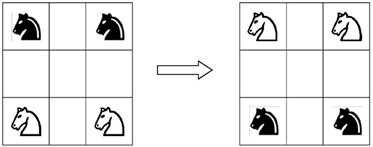
\includegraphics[keepaspectratio=true,scale=0.6]{HW1.jpg}}
\captionof{figure}{Start to Goal board state}    
\end{minipage}

\vspace{0.5cm}
\noindent The Four Knights puzzle is played on a 3 by 3 chess board. As depicted in \textit{Figure 1}, the opposing knights (two white and two black) begin in opposite corners. The goal of this puzzle is to have the opposing knights switch sides of the three-by-three chess board. The knights are moved one at a time, using the standard movement rule (two squares ahead in any direction, then one square left or right).
\newpage
\section{Data Structure}

\noindent The environment is represented by a chessboard with two white knights (W) and two black knights (B). The initial state of the chessboard is as follows:

\[
\begin{array}{ccc}
 B & . & B \\
 . & . & . \\
 W & . & W \\
\end{array}
\]

\noindent The goal is to find the shortest path from the initial state to a goal state. The goal state is represented by the following configuration of the chessboard:

\[
\begin{array}{ccc}
 W & . & W \\
 . & . & . \\
 B & . & B \\
\end{array}
\]

\noindent These environments, or board states, are stored in a class, \texttt{ChessBoard},  with attributes to track who's turn it is and lists of coordinate positions of each knight.  These \texttt{ChessBoard} objects are nested into a \texttt{Node} class.  

\noindent The \texttt{Node} class facilitates the relationship between \texttt{ChessBoard} objects.  The attributes in the \texttt{Node} include a \texttt{ChessBoard} object for the board, scoring values to hold costs of the \texttt{Node} in relation to the tree, a \texttt{parent} \texttt{Node} object, and a list of \texttt{children} \texttt{Node} objects.  Methods in this class are to generate valid child \texttt{Node}s and calculate scoring.
\newpage

\section{Algorithm Implementations}
\subsection{A* Implementation}
\noindent The full implementation of the A* search algorithm can be found in the accompanying \texttt{.py} file. The breakdown of how the A* algorithm is implemented is as follows:

\begin{python}
open_list: list[Node] = [Node()]
closed_list: list[Node] = []
\end{python}

\noindent These two lists are to act as a queue of \texttt{Node}s to evaluate and a list of nodes that have previously been evaluated. Following this is the main \texttt{while} loop to build and iterate over the tree.
\vspace{0.4cm}
\begin{python}
while open_list:
    currentNode = min(open_list, key=lambda node: node.f_score)
    open_list.remove(currentNode)
    currentNode.make_children()
    for child in currentNode.children:
\end{python}

\noindent The section above begins and continues the \texttt{while} loop so long as the queue has a \texttt{Node} in it.
The algorithm will then find the \texttt{Node} with the smallest \texttt{f} value, remove it from the queue, and generate it's child \texttt{Node}s.  After which, the algorithm will begin iterating over those children performing 2 main tasks:
\newpage
\begin{python}
if child.board.boardState == goalState.board.boardState:
    optimalPath = [goalState]
    while currentNode is not None:
        optimalPath.append(currentNode)
        currentNode = currentNode.parent
    return optimalPath[::-1]
\end{python}
\noindent The first task is to check if the \texttt{child}'s \texttt{boardState} is equivalent to the goal \texttt{boardState}. 
If it is then the algorithm will walk back up the tree by logging the \texttt{Node} into a list and stepping to each \texttt{parent} until it reaches the initial \texttt{Node} with no \texttt{parent}.  Returning the inverted list will return a list ordered from initial \texttt{boardState} to goal \texttt{boardState}.
\vspace{0.4cm}
\begin{python}
child.calc_heuristic()
i = find(child, open_list)
if not (i != -1 and open_list[i].f_score < child.f_score):
    i = find(child, closed_list)
    if not (i != -1 and closed_list[i].f_score < child.f_score):
        open_list.append(child)
\end{python}

\noindent The second task will occur if the \texttt{child}'s \texttt{boardState} was not equivalent to the goal \texttt{boardState}.
In this event the algorithm will then calculate the \texttt{child}'s heuristic scores and compare it to the \texttt{Node}s in the queue and the list of \texttt{Node}s that have been evaluated.  If it is found to be a novel \texttt{Node} or a known \texttt{Node} with a lower cost than an evaluated equivalent \texttt{Node} then it will be added to the queue of \texttt{Node}s to evaluate. 
\vspace{0.4cm}
\begin{python}
closed_list.append(currentNode)
\end{python}

\noindent After the \texttt{for} loop of the children this final line within the \texttt{while} loop takes the \texttt{currentNode} and adds it to the list of \texttt{Node}s that have been evaluated.
If the algorithm exits the \texttt{while} loop without returning a discovered path it will return a string stating that no path was found.
\newpage
\subsection{Branch and Bound Implementation}
The full implementation of the Branch and Bound search algorithm can be found in the accompanying \texttt{.py} file. The breakdown of how the Branch and Bound algorithm is implemented is as follows:

\begin{python}
open_list: list[Node] = [Node()]
closed_list: list[Node] = []
shortestPath = []
shortestPathLength = float('inf')
\end{python}

\noindent The first two lists are to act as a queue of \texttt{Node}s to evaluate and a list of nodes that have previously been evaluated. 
The next two lists are to store the shortest path that has been discovered and it's length.  These are separate to initialize the length as infinitely high and use it as a bound for the best path.
Following this is the main \texttt{while} loop to build and iterate over the tree.
\vspace{0.4cm}
\begin{python}
while open_list:
    currentNode = open_list.pop(0)
\end{python}

\noindent The section above begins and continues the \texttt{while} loop so long as the queue has a \texttt{Node} in it. The algorithm will then \texttt{pop} the \texttt{Node} at the front of the queue.
The algorithm will perform 2 main tasks on the popped \texttt{Node}:

\begin{python}
if currentNode == goalState:                                                  
path = []
while currentNode is not None:
    path.append(currentNode)
    currentNode = currentNode.parent
if len(path) <= shortestPathLength:
    shortestPathLength = len(path)
shortestPath = path[::-1]
\end{python}
\newpage
\noindent The first task is to check if the \texttt{currentNode}'s \texttt{boardState} is equivalent to the goal \texttt{boardState}. 
If it is then the algorithm will walk back up the tree by logging the \texttt{Node} into a list and stepping to each \texttt{parent} until it reaches the initial \texttt{Node} with no \texttt{parent}.  Storing the inverted list will store a list ordered from initial \texttt{boardState} to goal \texttt{boardState} in the \texttt{shortestPath} list.
\vspace{0.4cm}
\begin{python}
else:                                                                               
    if currentNode.g_score + 1 < shortestPathLength:
        currentNode.make_children()                                                 
        for child in currentNode.children:
            i = find(child, open_list)                                              
            if i == -1 and child.g_score < shortestPathLength:
                i = find(child, closed_list)                                        
                if i == -1:
                    open_list = [child] + open_list 
\end{python}

\noindent The second task will occur if the \texttt{currentNode}'s \texttt{boardState} was not equivalent to the goal \texttt{boardState}.
In this event the algorithm will then compare the \texttt{currentNode}'s spent cost (\texttt{g}) to the \texttt{shortestPathLength}.  
If the current cost of arriving at this \texttt{Node + 1} is greater than the \texttt{shortestPathLength} it can be determined to be a worse path and therefore ignored.  If the current cost of arriving at this \texttt{Node + 1} is less than the \texttt{shortestPathLength} we will generate its child \texttt{Node}s. After which, the algorithm will begin iterating over those children to evaluate if they must be added to the queue.
If the \texttt{child} is found to be a novel \texttt{Node} or a known \texttt{Node} with a lower cost than the shortest path then it will be added to the front queue of \texttt{Node}s to evaluate.
\newpage

\begin{python}
if open_list:
    mNode = min(open_list, key=lambda node: node.g_score)                           
    if mNode != open_list[0]:                                                      
        open_list.remove(mNode) 
        open_list = [mNode] + open_list
closed_list.append(currentNode)
\end{python}

\noindent After the \texttt{for} of the children we check if the recent \texttt{pop} emptied the queue. If there are still \texttt{Node}s in the queue then find the one with the lowest spent cost (\texttt{g}) and move it to the front of the queue to be evaluated next.  Finding the minimum node is faster than sorting the entire queue each time.
The final line within the \texttt{while} loop takes the \texttt{currentNode} and adds it to the list of \texttt{Node}s that have been evaluated.
\vspace{0.4cm}
\begin{python}
if shortestPath:
    return shortestPath
else:
    return "no path found"
\end{python}

\noindent When the algorithm exits the while loop if a path was found it will be stored in the \texttt{shortestPath} list and thus returned.  If the \texttt{shortestPath} list is empty then no path was found and a string stating that no path was found will be returned.
\newpage

\section{Heuristic Calculation}

The full implementation of the \texttt{calc\_heuristic()} function can be found in the accompanying \texttt{.py} file.
The breakdown of how the heuristics are calculated are as follows:
\begin{python}
d1 = abs(whiteKnight[0]-0) + abs(whiteKnight[1]-0)
d2 = abs(whiteKnight[0]-0) + abs(whiteKnight[1]-2)
\end{python}

\noindent First, the distance from a knight to each destination is calculated.
\vspace{0.4cm}
\begin{python}
if d1 == 0:
    d1 = 4
elif d1 == 4:
    d1 = 2
if d2 == 0:
    d2 = 4
elif d2 == 4:
    d2 = 2
\end{python}

\noindent The distances are adjusted for edge cases to allow the calculation to function properly.
\vspace{0.4cm}
\begin{python}
whiteH += abs(d1 - 4) + abs(d2 - 4)
\end{python}

\noindent The heuristic calculation takes the inverse of the distances by subtracting 4 to best predict the cost of arrival at a destination.
This calculation is performed for each knight.  The example given was for the White knights however similar actions are taken for the Black knights.
\vspace{0.4cm}
\begin{python}
self.h_score = (whiteH + blackH)*2
self.f_score = self.g_score + self.h_score
\end{python}
\noindent After the heuristic for each side is calculated, it is then summed with the other side, and finally multiplied.  This is done to more greatly prioritize nodes that have been visited over exploring novel nodes.  Then each score is update for the given \texttt{Node}.
\newpage

\section{Results}
Both algorithms found an optimal path of 16 moves however the runtimes between the two algorithms were significantly different.
\begin{center}
\begin{tabular}{|p{4cm}|p{4cm}|}
\hline
\textbf{A*} & \textbf{Branch and Bound} \\
\hline
3ms & 12ms \\
\hline
3ms & 11ms \\
\hline
4ms & 11ms \\
\hline
3ms & 11ms \\
\hline
4ms & 11ms \\
\hline
3ms & 12ms \\
\hline
3ms & 12ms \\
\hline
3ms & 12ms \\
\hline
4ms & 12ms \\
\hline
4ms & 11ms \\
\hline
\end{tabular}
\end{center}
\noindent The A* search algorithm ran for an average of 3.4ms over 10 runs.

\noindent The Branch and Bound Algorithm ran for an average of 11.5ms over 10 runs.

\noindent A* search took 29.57\% of the runtime of Branch and Bound search to find an equally optimal solution.

\newpage
\begin{multicols}{2}
\noindent A* search example path:

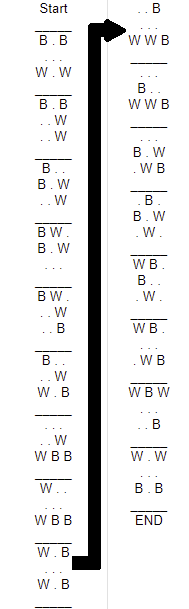
\includegraphics[scale=1]{AStarPath.png}
\vfill\null
\noindent Branch and Bound search example path:

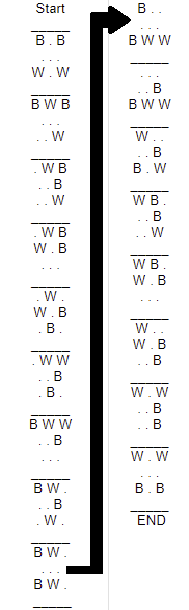
\includegraphics[scale=1]{bnbPath.png}
\end{multicols}
\newpage

\section{Conclusion}
While the A* search algorithm and the Branch and Bound search algorithm both found equally optimal paths from the initial state to the goal state, A* search completed the task significantly faster.  Were a more complex problem provided Branch and Bound may have been able to show its strength in finding a more optimal solution at the cost of time.  However, because the optimal solution was found through both algorithms and A* search preformed quicker, it can be concluded that A* search was better suited to solve this problem.

\end{document}